\subsection{Age of Empires}
Das Spiel \textit{Age of Empires} ist ein von \textit{Ensemble Studios} entwickeltes und von \textit{Microsoft} publiziertes, historisches Echt-Zeit-Strategie-Spiel für Einzel- und Mehrspieler, welches in Amerika im Jahr 1997 erschien. Die verwendete \textit{game engine} ist \textit{Genie}, welche hauptsächlich 2D \textit{sprites} verwendet \cite{aoe}. Age of Empires ist dabei der erste Teil der Reihe, mit drei weiteren Nachfolgern \textit{Age of Empires II, Age of Empires III} und \textit{Age of Empires IV}, und einem Ableger mit mythologischem Hintergrund \textit{Age of Mythology} \cite{aoe2}. Das Spiel wird in einer isometrischen Perspektive dargestellt (vgl. \autoref{image:aoe}). Es gibt verschiedenste Ressourcen und Einheiten, welche verschiedene Taktiken ermöglichen mit wiederum verschiedenen Konterstrategien. Ressourcen sind dabei finit, was bedeutet, dass ein gefällter Baum nicht wieder nachwachsen wird. Eine Kernkomponente des Spiels sind die verschiedenen Zeitalter, in welche der Spieler voranschreiten kann. Damit werden jeweils neue Technologien und Einheiten freigeschaltet, welche auf dem Weg zum Sieg hilfreich sein könnten. Die Zeitalter gliedern sich dabei auf in \textit{Altsteinzeit}, \textit{Jungsteinzeit}, \textit{Bronzezeit} und \textit{Eisenzeit} \cite*[]{aoe}. Es gibt dabei 12 verschiedene Völker, die an historische Völker angelehnt sind. Diese sind \textit{Ägypter, Assyrer, Babylonier, Chosonen, Griechen, Hethiter, Minoer, Perser, Phönizier, Shang, Sumerer} und \textit{Yamato}. Dabei hat jedes Volk eine andere Gesamtauswahl aus dem Technologiebaum. Alle wichtigen Eckdaten zu dem Spiel sind in \autoref{table:aoe} einsehbar.
\paragraph*{Siegbedingungen}
\begin{itemize}
    \item Alle Gegenspieler eliminieren mittels Militär
    \item Alle \textit{Artefakte} / Runen erobern
    \item Ein \textit{Weltwunder} bauen und erfolgreich bis Ende verteidigen
\end{itemize}

\paragraph*{Ressourcen}
\begin{itemize}
    \item Nahrung
    \item Holz
    \item Stein
    \item Gold
\end{itemize}\cite*[]{aoe:ressources}
\newparagraph{Rezensionen}
\begin{tabularx}{0.8\textwidth} { 
    | >{\raggedright\arraybackslash}X 
    | >{\centering\arraybackslash}X 
    | >{\raggedleft\arraybackslash}X | }
   \hline
   PC Games & 93\% \cite*[]{aoepcgames}\\
   \hline
   PC Player & 5/5 \cite*[]{aoepcplayer}\\
  \hline
  Power Play & 84\% \cite*[]{aoepowerplay}\\
  \hline
  GameRankings & 87,1\% \cite*[]{aoegamerankings}\\
  \hline
  IGDB & 85\% \cite*[]{aoe}\\
  \hline
\end{tabularx}

\begin{table}[]
    \centering
    \caption{Age of Empires Eigenschaften (\cite*[]{aoe,aoe:ressources,aoe2, aoe:technologies})}
    \label{table:aoe}
    \begin{tabular}{|l|l|}
    \hline
    Erscheinungsjahr & 1997                              \\ \hline
    Entwickler       & Ensemble Studios                  \\ \hline
    Publisher        & Microsoft                         \\ \hline
    Multiplayer        & Ja                         \\ \hline
    Ressourcen       & Nahrung, Holz, Stein, Gold        \\ \hline
    Siegbedingungen  & Domination, Artefakte, Weltwunder \\ \hline
    Spielbare Völker & 12                                \\ \hline
    Perspektive      & Isometrisch                       \\ \hline
    Technologien     & 53                                \\ \hline
    \end{tabular}
    \end{table}


\begin{figure}
    \begin{center}
        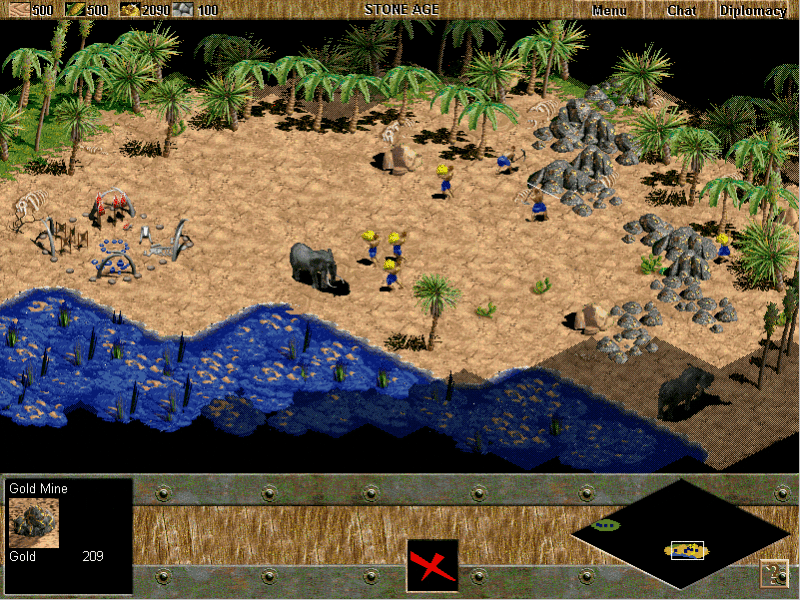
\includegraphics[width=300px]{0.bilder/aoe.png}
    \end{center}
    \caption{Screenshot aus Age of Empires (\cite{aoe})} \label{image:aoe}
\end{figure}